\section{ドイツでも寮食のタコライスが食べたい！}
\rightline{（文責：午後三時）}

農学部森林科学科4回生の午後三時です。去年1年間ドイツのゲッティンゲンに交換留学に行っていました。留学先の大学は食堂があり、京大の生協食堂よりも安くてヴィーガンやベジタリアンなどいろいろなメニューがあったのでそこまで食事には困らなかったのですが、ドイツには安い外食チェーンがあまりないこともあり、よく自炊もしていました。
以下は留学中に書いていた日記の中の「最近の自炊セレクション」という回から抜き出してきたものです。留学中、Twitterの熊野寮寮食botなどを見ながらたまに寮食が食べたくなっていました。帰ってきて、あの時食べたかった昼寮食のタコライスを食べられてうれしいです。息抜きにゆるく読んでもらえればと思います。

\subsection{2025/7/1 最近の自炊セレクション}

\subsubsection{5/30(金)タコライス風タコライス}
寮食のタコライスがおいしそうで食べたかった。しかし生肉を扱いたくない、ソイミートのひき肉は少し割高、ご飯を鍋で炊くのはめんどくさい、という理由からレンズ豆にツナを混ぜてひき肉風に、少し前に買ったクスクスをご飯の代わりにした。かなりおいしかった！私がタコライスに求めていたものは何となくすべて満たされた。

\begin{figure}[h]
  \centering
  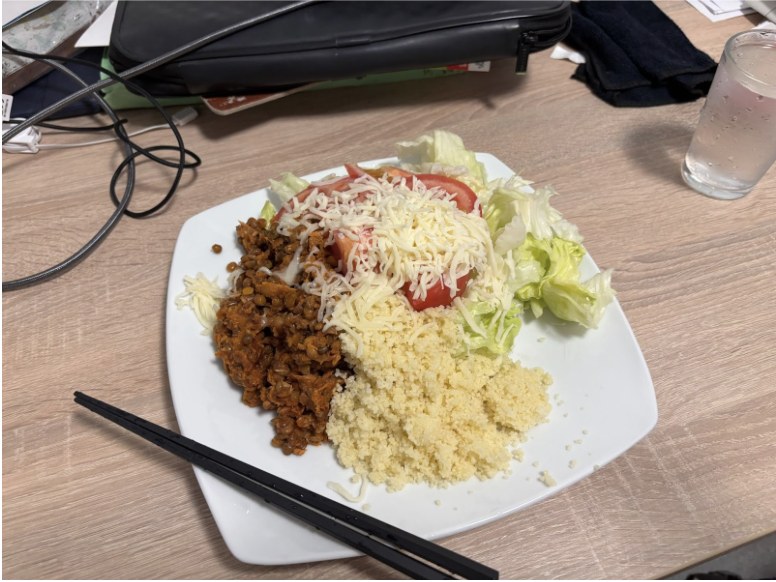
\includegraphics[width=0.8\linewidth]{2026shinki/tacos_in_german/images/TacoRice.png}
  \caption{タコライス風タコライス}
\end{figure}

\subsubsection{6/28(土) ルバーブの梅そうめん風スパゲティ}

ドイツで春に見かけるルバーブというピンク色の野菜がある。酸味があって、ジュースやジャムにするらしい。以前大学の日独タンデム会で他の人が飲んでいた。そろそろ季節が終わりそうだったので一度食べてみたくて買って、半分はジャムにした。塩もみをして煮詰めることで梅干し風ペーストになると言っているブログがあったので残りの半分でそれを試してみた。
(ルバーブの他の食べ方について：生→酸っぱい、シュウ酸？みたいな味がする。生で食べるものではない。ジュース：まあまあ。私が買ったジュースはあまり甘くなくてちょっと酸っぱいくらいで特に野菜の味がする。ジャム：おいしい！おいしかったけどルバーブそれ自体に甘みはほぼないのでかなり砂糖を入れてちょうどいい感じ。ルバーブの酸味と砂糖の甘みの味)
作った梅干し風ルバーブペーストを凍らせて、ツナ、ネギと一緒に細めのスパゲッティに乗せ、めんつゆを買うのがめんどくさいので醤油をかけた。見た目がかなり梅干しのペーストっぽくて面白い。繊維感がちょっと残っているところとか。味は100\%梅とはいかないが酸味と塩味があってこの見た目ならかなり梅だと思う。はちみつ梅よりはしそ梅に近い。梅風味にありがちな不思議な香りとかは無い。ちょっと手間はかかるが和風感あっておいしかった！もうルバーブは売っていないので再現できないのは残念。

\begin{figure}[h]
  \centering
  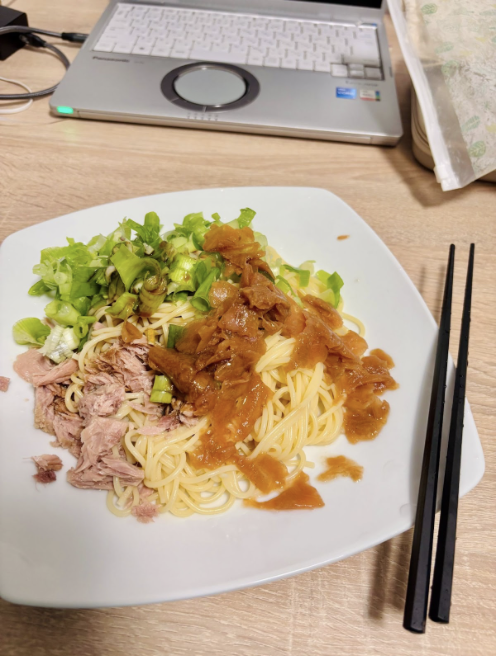
\includegraphics[width=0.8\linewidth]{2026shinki/tacos_in_german/images/Spaghetti.png}
  \caption{ルバーブの梅そうめん風スパゲティ}
\end{figure}
 
\subsubsection{6/29(日)　シュパーゲルのオランデーソース添えとアンズタケとシュパーゲルのリゾット}

シュパーゲル(Weißer Spargel白アスパラ)もドイツの春の代表的な味覚。4月ごろから市場やスーパーに出始め、根？を休めるために6/24の聖ヨハネの日でほぼ採取・販売が終了する。以前食べておいしかったので最後にもう一度食べたいと思って買ってきていた。
またアンズタケ(Pfifferling)は夏から秋に書けて出回る少し高級なきのこであんずのような香りがすることからアンズタケと呼ばれるらしい。ドイツ語Pfifferlingは味の方から来ていて胡椒っぽい味と言われている。生と加熱で食べてみたが、香りも味もわかるようなわからないような。
シュパーゲルはゆで汁にだしが出るからゆで汁も有効活用したほうが良いと言われていて、前回はインスタントのシュパーゲルスープを戻すときのお湯につかってみた。リゾットにしているレシピもあったので、今回はリゾットで使うお湯にゆで汁を使った。きのこのほうもクリーミーな料理が合うと書いてあり、リゾットにしているレシピもあった。オリーブオイルできのことにんにくとご飯を炒め、シュパーゲルのゆで汁とシュパーゲルの繊維感の強い下の方の部分を少しいれ、最後に牛乳とチーズも入れて胡椒をかけた。めちゃくちゃおいしかった。
シュパーゲルとオランデーソースの組み合わせで食べるのはもう3回目なので味がわかっていると言ってもやはりおいしい。リゾットの方はあまりレシピを見ずに適当に作った割にはかなり自分の中では深みのある本格的な味がして本当においしかった。あとリゾットはご飯を鍋で炊くデメリットの底につく、浸水がめんどくさいなどを解消できるのもよいと思った。他の日に作ったルッコラのオランデーソースのパスタもおいしかった。ちょっとクリームソースっぽくなる。

\begin{figure}[h]
  \centering
  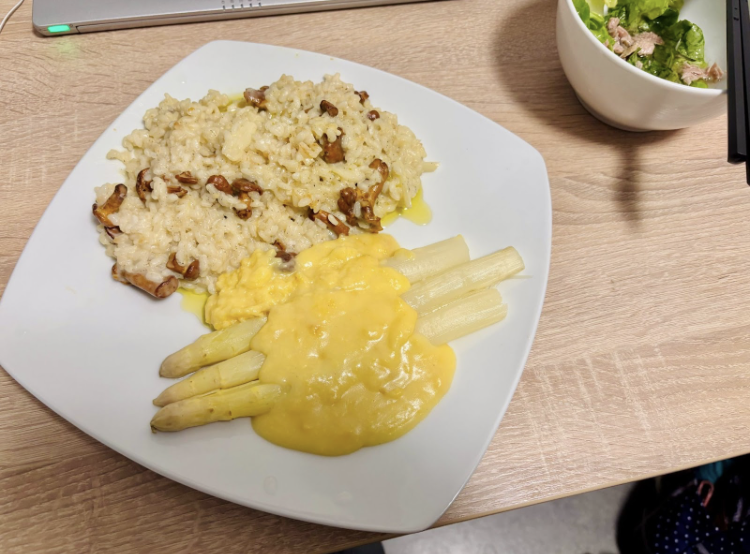
\includegraphics[width=0.8\linewidth]{2026shinki/tacos_in_german/images/Risotto.png}
  \caption{シュパーゲルのリゾット}
\end{figure}
 
\subsubsection{6/30(月) レンズ豆となすのドライカレー風}

ナスが安くて大きいのに2個で1€くらいだった。乾燥レンズ豆を戻してナス、にんにく、トマトペーストなどと炒め、カレー粉、胡椒、チリパウダーなどで味付けした。ドイツにはTomaten Markというトマトの濃縮ペーストのようなものが金属のチューブに入って売っている。ケチャップも売っているが、これはケチャップのように味がついているわけではなくそのままトマトの味がする。また同じような金属のチューブでsenfという名前でマスタードもよく売っている。全然使わなくて余っているのでマスタードも少しだけ入れてみた。あとネギも入れてみた。理想のいい感じのバランスの味にできて満足。豆を使うと炭水化物以外でボリュームが出せるのがいい。ご飯の代わりにクスクスを合わせた。おいしかった。

\subsection{ドイツの生活と熊野寮の共通点}

ドイツでは家賃がかなり高騰しているため学生で一人暮らし人は少なく、たいてい大学寮またはWG(Wohngemeinschaft)というシェアフラットのようなところに住んでいます。私の留学先の大学寮はその中間みたいな感じで、それぞれ個室があり4人でキッチンやシャワートイレを共有していました。人と一緒に住んでいて困ることはどこでも多少似ているので、熊野寮でもこういうことあったなという気持ちになることが多かったです。キッチンに洗ってない食器を放置しないでとか、同じ人がずっとゴミ出しをしているから当番を決めようとか。
熊野寮は家賃が安くて貯金しやすいだけでなく、人と一緒に住む経験ができるのもいいところだと思います。400人以上もいるので実際にどういう人が住んでいるのか外からではわかりにくいし不安もあると思いますが、このパンフで少しでもこんな人が住んでるんだというのが伝わればうれしいです。見学もやっているのでよかったら来てみてください。寮食は寮外生の方でも寮生と友達になれば食べられるので、寮に入っても入らなくても食べてみてください。タコライスもおいしいしタコライス以外ももちろんおいしいです。
冬のゲッティンゲンは京都よりも天気が悪く曇り空が続きます。しかし春になると一転して青空が広がり、ゲッティンゲン大学の中央キャンパスの桜並木ではまさにFrühling(春)!と言いたくなるような美しい景色になります。もし入試の前とか1日目の夜とかにこのパンフを開いてここを読んだ珍しい人がいたら、（その気持ちの余裕があるならたぶん大丈夫ですが）応援しています。あなたが後悔なく受験を終えて、素敵な春を迎えられることを願っています。